\chapter{Implementation} 

%%%%%%%%%%%%%%%%%%%%%%%%%%%%% Introduction %%%%%%%%%%%%%%%%%%%%%%%%%%%%%

\section*{Introduction}

This chapter describes the implementation details of the Collaborative Highway Surveillance (CHS) system developed for real-time detection of speeding violations. It presents the tools, libraries, and development environments used to build, integrate, and test the communication modules, routing logic, and prediction components. Special attention is given to the configuration and synchronization of UAVs and ground nodes, ensuring stable data exchange and minimal latency across the network.

Next, we detail the development of the communication protocol, combining MAVLink for drone-to-drone and drone-to-ground communication with UDP for lightweight sensor data transmission. The distributed drone selection algorithm is implemented to account for residual energy, proximity to target zones, and avoidance of redundant coverage.

We then describe the integration of the machine learning prediction module, trained on historical and simulated speeding data to anticipate infraction hotspots. The implementation ensures that computationally heavy operations are executed on ground stations when possible, preserving UAV autonomy.

The final section focuses on system optimization, including strategies for reducing energy consumption, improving communication reliability, and achieving a balance between real-time responsiveness, processing requirements, and operational scalability.

%%%%%%%%%%%%%%%%%%%%%%%%%%%%% Choice of Physical Material %%%%%%%%%%%%%%%%%%%%%%%%%%%%%

\section{Choice of Physical Material}

Before selecting drones for experimentation, it is crucial to clearly define the operational requirements. 
Deploying a drone-based surveillance infrastructure requires consideration of both technical and 
regulatory constraints associated with the equipment. In order to choose suitable drones, several 
selection criteria were evaluated as presented in Table~\ref{tab:drone_criteria}.

\begin{table}[H]
\centering
\caption{Drone selection criteria}
\label{tab:drone_criteria}
\begin{tabular}{|p{4cm}|p{9cm}|}
\hline
\textbf{Criteria} & \textbf{Details} \\ \hline
Flight capabilities & Endurance, maximum speed, transmission range \\ \hline
Camera specifications & Resolution, low-light performance, overall image quality \\ \hline
Technical aspects & Ease of integration into the communication network, 
synchronization with protocols, compatibility with detection and obstacle-avoidance systems \\ \hline
Regulatory aspects & Compliance with national aviation regulations and safety standards, 
respect for privacy and data protection (e.g., EU directives) \\ \hline
Performance and reliability & User feedback, stability of performance, low maintenance requirements \\ \hline
Cost and budget & Operational expenses, financing options, availability of subsidies \\ \hline
Support and services & Availability of technical support, after-sales service, spare parts and repair facilities \\ \hline
Sustainability & Low environmental impact, long-term operational viability \\ \hline
\end{tabular}
\end{table}

Based on these requirements, three categories of drones were identified as particularly relevant:  
\begin{itemize}
    \item \textbf{Pixhawk/Ardupilot-based drones}: Open-source, modular, and programmable platforms, adaptable to mission needs.  
    \item \textbf{DJI Inspire 2}: Professional-grade, robust, and reliable in challenging environments.  
    \item \textbf{Holybro X500 V2 and Hexsoon EDU 450}: Highly flexible, supported by an active open-source community.  
\end{itemize}

\begin{figure}[H]  
    \centering
    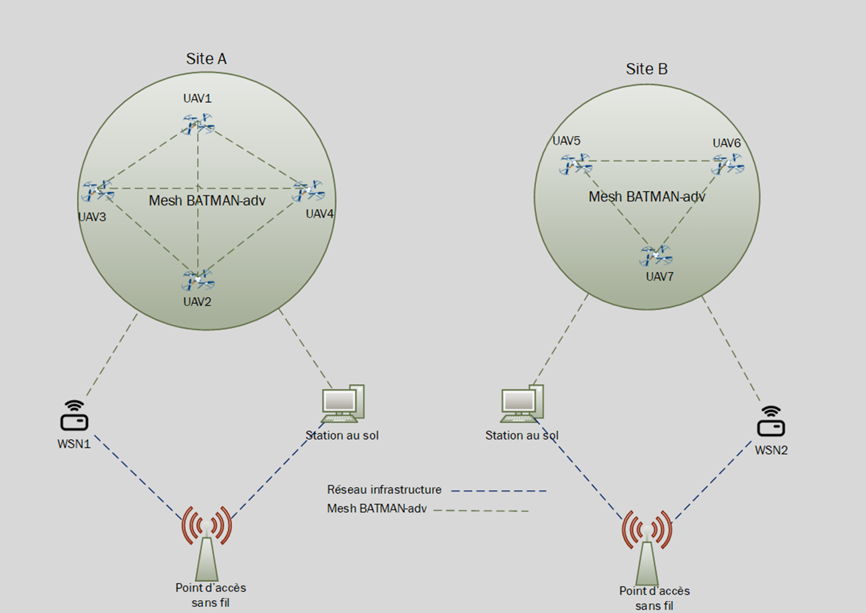
\includegraphics[width=1.0\textwidth]{Figures/Chapter5/Section2/archi.png} % Adjust width as needed
    \caption{Proposed CHS system architecture.}
    \label{fig:proposed_architecture} % Reference label
\end{figure}


The selection of drones for highway surveillance must therefore be guided by operational needs, 
technical and regulatory constraints, as well as economic and environmental considerations.  
Figure~\ref{fig:chs_architecture} illustrates the proposed system architecture.

\subsection*{Selection of Equipment}

The choice of supporting hardware was made according to both technical and financial constraints. 
Performance, reliability, and adaptability were identified as key criteria, which led us to select 
Pixhawk-based drones with the Ardupilot firmware.

\subsubsection*{Pixhawk-based Drones}

The Pixhawk 2.4.8 flight controller (Figure~\ref{fig:pixhawk}) was selected due to its high modularity.  
Pixhawk-based drones allow extensive hardware and software customization, making them suitable 
for this project. They are compatible with a wide range of sensors, communication modules, and 
navigation tools, enabling specific mission configurations while ensuring the desired performance.  
Pixhawk is an open-source flight controller developed by PX4 and supports both PX4 and Ardupilot 
autopilot software.

\begin{figure}[H]  
    \centering
    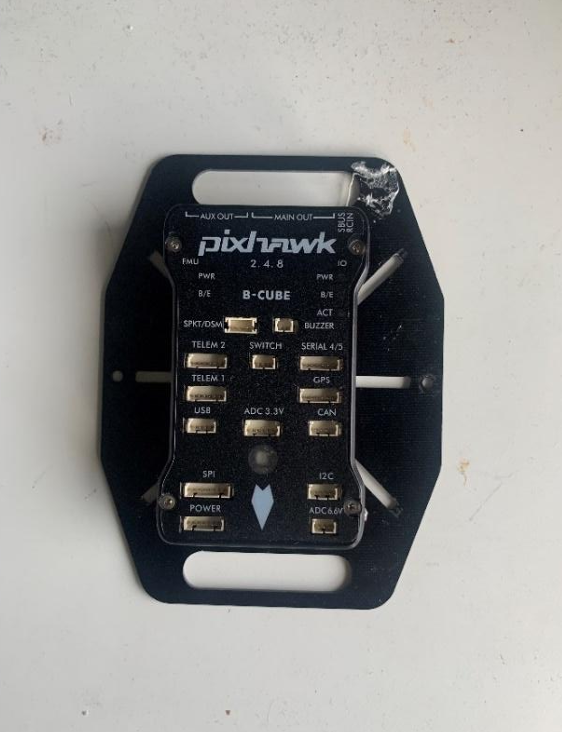
\includegraphics[width=0.5\textwidth]{Figures/Chapter5/Section2/pixhawk.png} % Adjust width as needed
    \caption{Proposed CHS system architecture.}
    \label{fig:proposed_architecture} % Reference label
\end{figure}


For the drone frames, we selected the \textbf{DJI F450} and \textbf{Turnigy SK450} (Figure~\ref{fig:frames}), 
equipped with the flight controller and necessary accessories to achieve autonomous flight.  
The complete hardware setup includes:  

\begin{itemize}
    \item Pixhawk PX4 2.4.8 flight controller  
    \item Ublox NEO-M8N GPS module for navigation and autonomy  
    \item 2212 920KV 30A brushless motors (2 CW, 2 CCW)  
    \item Multistar 20A ESCs (x4)  
    \item Propellers: 2 CW, 2 CCW  
    \item F450 frame: 450mm width, 55mm height, 280g (395g with accessories)  
    \item Raspberry Pi Zero 2 W for telemetry and mesh networking, also equipped with a camera  
    \item Raspberry Pi Camera module  
    \item Power Distribution Board (PDB) to manage power delivery and supply the Raspberry Pi  
    \item MicroSD card for flight data and system logs  
    \item LiPo batteries (Zeee 3S 2200mAh 11.1V 50C or 5200mAh 80C)  
    \item LiPo charger  
    \item Power module for battery monitoring by the flight controller  
\end{itemize}

\subsubsection*{Raspberry Pi Zero 2 W}

The Raspberry Pi Zero 2 W (Figure~\ref{fig:rpi}) is a single-board computer running Linux, 
widely used in IoT and embedded applications. With integrated Wi-Fi (2.4GHz) and Bluetooth 4.2, 
it can communicate with other devices in a network. Its GPIO pins support extensions such as sensors 
and modules, making it suitable for telemetry and onboard image capture in our drone setup.  

Its main specifications are:  
\begin{itemize}
    \item Broadcom BCM2710A1, quad-core Cortex-A53 64-bit 1GHz CPU  
    \item 512 MB LPDDR2 SDRAM  
    \item 2.4GHz 802.11 b/g/n Wi-Fi  
    \item Bluetooth 4.2 / BLE, integrated antenna  
    \item Mini HDMI, micro USB OTG  
    \item MicroSD card slot  
    \item CSI-2 camera connector  
    \item 40-pin GPIO header footprint  
    \item Micro USB power supply  
    \item Composite video and reset pins via test pads  
    \item H.264/MPEG-4 decoding (1080p30), H.264 encoding (1080p30)  
\end{itemize}

\begin{figure}[H]  
    \centering
    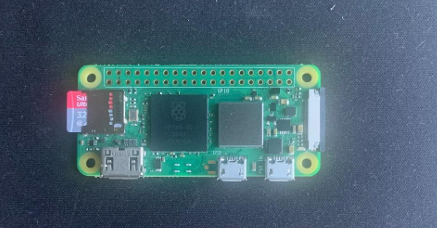
\includegraphics[width=0.5\textwidth]{Figures/Chapter5/Section2/pi2w.png} % Adjust width as needed
    \caption{Proposed CHS system architecture.}
    \label{fig:proposed_architecture} % Reference label
\end{figure}

\begin{figure}[H]  
    \centering
    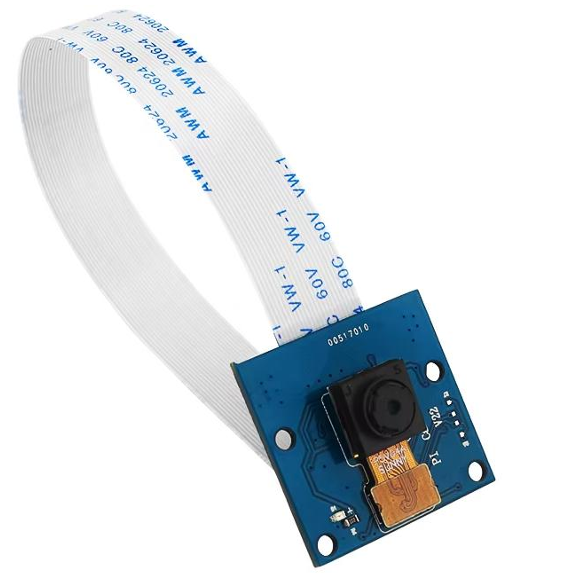
\includegraphics[width=0.5\textwidth]{Figures/Chapter5/Section2/camera.png} % Adjust width as needed
    \caption{Proposed CHS system architecture.}
    \label{fig:proposed_architecture} % Reference label
\end{figure}


%%%%%%%%%%%%%%%%%%%%%%%%%%%%% Choice of Tools and Development Environment %%%%%%%%%%%%%%%%%%%%%%%%%%%%%

\section{Choice of Tools and Development Environment}

The implementation of the Collaborative Highway Surveillance (CHS) system required a 
combination of programming languages, development tools, communication protocols, 
and machine learning frameworks. This section presents the main tools and environments 
used during the development process.

\subsection*{Programming Language}
The majority of the implementation was carried out in \textbf{Python}. This language was chosen 
for its flexibility, extensive libraries, and compatibility with both the Raspberry Pi and 
drone communication frameworks. Python was used to implement the communication 
protocols (UDP and MAVLink), the distributed decision-making algorithm, and 
the integration of computer vision and machine learning modules. 

\subsection*{Communication and Drone Control}
\begin{itemize}
    \item \textbf{MAVLink (Micro Air Vehicle Link)}: a lightweight messaging protocol 
    widely used in unmanned aerial systems for communication between drones, sensors, 
    and ground stations.  
    \item \textbf{PyMAVLink}: the Python implementation of MAVLink, used to encode and 
    decode messages exchanged in the system.  
    \item \textbf{UDP sockets}: implemented to support direct communication between 
    drones and ground nodes (RN/NH).  
    \item \textbf{Crazyflie Python API and Crazyradio}: employed during early testing 
    with Crazyflie drones before integration with Pixhawk-based platforms.  
\end{itemize}

\subsection*{Firmware and Flight Control}
The drones were equipped with the \textbf{Pixhawk 2.4.8 flight controller} running 
the \textbf{Ardupilot} firmware. Ardupilot was selected for its open-source nature, 
flexibility, and wide community support. It allowed the configuration of autonomous 
flight missions while ensuring compatibility with MAVLink. PX4 was also considered, 
but Ardupilot was retained as the primary firmware for this project.

\subsection*{Onboard Processing Environment}
For onboard processing, the \textbf{Raspberry Pi Zero 2 W} was integrated with the drones. 
This single-board computer ran \textbf{Raspberry Pi OS (Linux-based)} and hosted the 
Python scripts responsible for telemetry, communication with ground sensors, 
and computer vision tasks. Its Wi-Fi connectivity was used to establish a mesh 
network between drones.

\subsection*{Ground Control Software}
Two Ground Control Station (GCS) applications were used:  
\begin{itemize}
    \item \textbf{Mission Planner}: mainly for configuring Ardupilot parameters, 
    uploading missions, and monitoring telemetry.  
    \item \textbf{QGroundControl}: used as an alternative interface for visualization 
    and debugging of flight data.  
\end{itemize}

\subsection*{Machine Learning Tools}
Machine learning algorithms for predicting speed violations were developed 
using the following tools:  
\begin{itemize}
    \item \textbf{Scikit-learn}: for preprocessing, feature extraction, and classical ML algorithms 
    such as regression and classification.  
    \item \textbf{TensorFlow/PyTorch}: considered for advanced training tasks and 
    neural networks, particularly for handling more complex datasets.  
    \item \textbf{Jupyter Notebook}: used for prototyping, training, and analyzing 
    machine learning models.  
\end{itemize}

\subsection*{Computer Vision Tools}
To detect and validate speed violations using drone cameras, computer vision 
techniques were implemented with:  
\begin{itemize}
    \item \textbf{OpenCV}: for image preprocessing, frame extraction, and speed estimation 
    through motion analysis.  
    \item \textbf{YOLO (You Only Look Once)}: for real-time object detection and vehicle recognition, 
    enabling the system to detect vehicles directly from the drone’s onboard camera feed.  
    \item \textbf{Raspberry Pi Camera API}: for integrating the onboard camera with the 
    Raspberry Pi module.  
\end{itemize}

\subsection*{Collaboration and Documentation Tools}
For project management and documentation:  
\begin{itemize}
    \item \textbf{Git and GitHub}: for version control and collaborative development.  
    \item \textbf{LaTeX}: for the preparation and formatting of the thesis document.  
\end{itemize}




%%%%%%%%%%%%%%%%%%%%%%%%%%%%% Communication Protocol Implementation %%%%%%%%%%%%%%%%%%%%%%%%%%%%%

\section{Communication Protocol Implementation}

\subsection{Setting up the Mesh Network}

Typically, drones utilize the MAVLink protocol to exchange data with a ground station through a point-to-point radio link. In this setup, a drone communicates directly with a control station, often via a short-range radio connection. While this approach is efficient for single-drone communications with a ground station, it has limitations when multiple drones need to interact or share data in real-time.

To overcome these limitations and enable multi-drone communication, we opted for a mesh network. Unlike point-to-point links, where each drone connects individually to the ground station, a mesh network allows every drone to function as both a communication node and a data relay. This enables drones to forward information to other drones or the ground station via intermediate nodes, improving resilience and coverage. If a drone loses direct connectivity with the ground station, it can still transmit data through other drones.

We implemented this mesh network using Raspberry Pi modules, employing the BATMAN-adv protocol for dynamic routing within the ad-hoc network. These modules interconnect drones, speed sensors, and ground stations, forming a flexible and robust infrastructure (Figure~\ref{fig:test_platform}). Each sensor acts as a node in the mesh network and facilitates MAVLink message exchange between the mesh and infrastructure networks. The architecture isolates the drone network and introduces an additional security layer using native Linux policies.

\begin{figure}[h!]
\centering
\includegraphics[width=0.7\textwidth]{platform_test.png}
\caption{Test platform with BATMAN-adv interconnection between drones and ground stations.}
\label{fig:test_platform}
\end{figure}

\subsubsection{Installing Raspberry Pi on Drones}

Raspberry Pi modules are widely used to add advanced features to drones. We utilize them for telemetry, onboard camera, and speed sensor functions. Additionally, they serve as software bridges with MAVLink-router, connecting Pixhawk flight controllers to other network nodes.

For hardware installation, we used:
\begin{itemize}
    \item Raspberry Pi Zero 2 W;
    \item Dupont cables for connections;
    \item UART-to-USB converter for serial communication testing;
    \item 3S LiPo battery;
    \item Mission Planner ground station;
    \item Soldering equipment.
\end{itemize}

The Raspberry Pi is powered separately from the drone's main battery, connected directly to the PDB on the F450 frame (Figure~\ref{fig:pi_pixhawk}). Communication with the flight controller uses the UART serial interface (e.g., TELEM1, TELEM2), connecting telemetry modules like ESP32 or Raspberry Pi.

\begin{figure}[h!]
\centering
\includegraphics[width=0.7\textwidth]{pi_pixhawk.png}
\caption{Raspberry Pi connected to Pixhawk via UART.}
\label{fig:pi_pixhawk}
\end{figure}

Connections:
\begin{itemize}
    \item 5V Pi to 5V PDB;
    \item GND Pi to GND PDB;
    \item TX Pi to RX Pixhawk;
    \item RX Pi to TX Pixhawk.
\end{itemize}

\subsubsection{Overview of BATMAN-adv}

BATMAN-adv operates like traditional IP link-state protocols but in a decentralized manner. Each node only knows the next hop for data forwarding. Routing tables are built using ELP (Echo Location Protocol) to discover direct neighbors and OGMs (Originator Messages) to propagate routing information.

\begin{itemize}
    \item ELP identifies neighboring nodes and evaluates link quality.
    \item OGMs broadcast each node’s presence and routes, decrementing TTL as messages propagate.
\end{itemize}

Data is routed hop-by-hop, dynamically updating tables if nodes become unavailable, ensuring adaptation to network topology changes.

\subsubsection{Mesh Network Configuration}

Raspberry Pi modules on drones are configured as follows:
\begin{enumerate}
    \item Install OS on microSD using Raspberry Pi Imager (preferably headless).
    \item Enable UART port and disable Bluetooth via \texttt{/boot/firmware/config.txt} and \texttt{systemctl}.
    \item Configure the infrastructure network (\texttt{wlan1}) using \texttt{wpa\_supplicant}.
    \item Install BATMAN-adv: \texttt{sudo apt install batctl wireless-tools iptables ifupdown -y}.
    \item Set up interfaces in \texttt{/etc/network/interfaces}, assigning static IP to \texttt{bat0}.
    \item Create startup scripts for \texttt{bat0} configuration to ensure persistence after reboot.
    \item Verify network using ARP tables, neighbors, client/server mode, routing tables, and OGM capture.
\end{enumerate}

\subsubsection{Software Bridge Integration}

MAVLink-router is installed on the Raspberry Pi to route MAVLink messages from the drone's UART to the mesh network:
\begin{itemize}
    \item Disable console on serial port via \texttt{raspi-config}.
    \item Set up Python virtual environment and install \texttt{mavlink-router, pymavlink, pyserial}.
    \item Remove conflicting packages like \texttt{ModemManager}.
    \item Compile and install MAVLink-router from source, allowing message distribution between Pixhawk and multiple clients via TCP/UDP.
\end{itemize}




\subsection{Collecting Local UAV Data}

In order to monitor and record the state of the UAV, a dedicated local data collection mechanism has been implemented using Python and MAVProxy. This subsystem is responsible for interacting with the drone’s autopilot through the MAVLink protocol and extracting key status information in real time.

\subsubsection{MAVProxy Integration}

The core of this process relies on \texttt{mavproxy.py}, which serves as a middleware to communicate with the flight controller. The script launches MAVProxy using a serial connection (\texttt{/dev/serial0}) with a baud rate of 57600. Once the connection is established, the script sends a \texttt{status} command to request the UAV’s telemetry and status information. This approach ensures that all essential onboard parameters are captured without interfering with normal flight operations.

\subsubsection{Output Retrieval and Timing}

After sending the \texttt{status} command, the script reads the MAVProxy output line by line over a five-second interval. This mechanism captures a snapshot of the UAV’s current state. A timeout is implemented to prevent indefinite blocking in case the UAV does not respond or the connection is unstable. The retrieved raw output is stored for further parsing and processing.

\subsubsection{Parsing MAVLink Messages}

Raw MAVLink messages are structured but often include multiple fields with varying data types. The script implements a custom parser that:

\begin{itemize}
    \item Uses regular expressions to extract key-value pairs from the MAVLink messages.
    \item Converts numeric values to appropriate Python types (\texttt{int} or \texttt{float}).
    \item Handles arrays and special string formats.
    \item Annotates each message with a timestamp for temporal context.
\end{itemize}

This parsing step transforms unstructured MAVLink text output into a well-organized dictionary format, where each message type (e.g., \texttt{HEARTBEAT}, \texttt{SYS\_STATUS}) can contain multiple entries representing the UAV’s current state.

\subsubsection{Data Aggregation}

Once parsed, messages are grouped by type into a single \texttt{messages} dictionary. This allows for efficient indexing and retrieval of specific data points. For example, battery status, GPS position, or system health can be accessed independently without scanning the raw output.

\subsubsection{Verification and Output}

Finally, the processed data is displayed in JSON format, providing a concise view of the UAV’s current state. This visualization serves both as a debugging tool and a verification step to ensure the integrity of collected information. The use of JSON also facilitates downstream tasks such as logging, analysis, or transmission over a communication protocol.




\subsection{UAV-to-UAV Status Exchange via MAVLink}

To enable cooperative operation and real-time situational awareness among multiple UAVs, a communication module for exchanging UAV status information was implemented. This module uses the MAVLink protocol to transmit structured telemetry data from one UAV to another, ensuring that each UAV can be aware of the state of its peers. The implementation is divided into a sender and a receiver component.

\subsubsection{Sender Implementation}

The sender component retrieves the local UAV status from onboard sensors and systems using the \texttt{get\_uav\_status\_data()} function. This status data typically includes:

\begin{itemize}
    \item UAV identification number
    \item Geographic position (latitude, longitude)
    \item Altitude
    \item Battery level
    \item Speed
    \item System status
    \item Timestamp of the measurement
\end{itemize}

To send this information reliably over MAVLink, the data is first serialized into a JSON string. Because MAVLink \texttt{STATUSTEXT} messages have a limited payload size, the JSON string is split into smaller chunks of 35 characters each. The sending protocol then follows these steps:

\begin{enumerate}
    \item \textbf{Start marker:} A \texttt{STATUS\_START} message is sent, including metadata about the total number of chunks and the total message length.
    \item \textbf{Data chunks:} Each chunk is transmitted in sequence using \texttt{STATUS\_PART} messages with explicit sequence numbers.
    \item \textbf{End marker:} A \texttt{STATUS\_END} message signals the completion of the transmission.
\end{enumerate}

This structured transmission ensures that the receiving UAV can correctly reconstruct the full JSON payload even if messages arrive out of order or experience delays.

\subsubsection{Receiver Implementation}

The receiver continuously listens for incoming \texttt{STATUSTEXT} messages. Upon receiving a \texttt{STATUS\_START} message, it initializes a temporary buffer and expects a specific number of chunks. As \texttt{STATUS\_PART} messages arrive, the receiver stores them in a dictionary indexed by sequence number. Once the \texttt{STATUS\_END} marker is received and all chunks are present, the JSON string is reconstructed, verified for length consistency, and parsed back into structured data. The timestamp field is converted back into a Python \texttt{datetime} object for temporal tracking.

Finally, the received status can be displayed for verification or stored in a database using existing functions such as \texttt{save\_uav\_status\_db()}. This allows real-time monitoring of peer UAVs and provides a foundation for cooperative decision-making or swarm coordination.

\subsubsection{Reliability and Timing Considerations}

A small delay of 0.1 seconds is introduced between sending consecutive chunks to avoid message collisions or overload on the communication link. The receiver includes a timeout mechanism (default 5 seconds) to prevent indefinite blocking if some chunks are lost. Errors in decoding, incomplete transmissions, or malformed messages are logged, ensuring robustness in real-world operations.



\subsection{Simulated Speed Record Generation}

In order to test and validate the UAV monitoring system without relying solely on real-world flight data, a simulation module for generating speed records was implemented. This module produces synthetic UAV speed measurements over time, including both normal and threshold-violating values, enabling controlled testing of data processing, alerting, and database storage mechanisms.

\subsubsection{Configuration and Thresholds}

The simulation reads a configuration file (\texttt{config.json}) containing a \texttt{violation\_threshold} parameter, which defines the upper limit for normal UAV speed. Any simulated speed exceeding this threshold is considered a violation, which can be used to trigger alerts or log incidents. The simulation also uses hardcoded generation parameters for the speed range and the interval between measurements:

\begin{itemize}
    \item Minimum speed: 60 km/h
    \item Maximum speed: 210 km/h
    \item Violation probability: 30\% of the measurements
    \item Measurement interval: 2 to 5 seconds
\end{itemize}

\subsubsection{Speed Generation Logic}

The \texttt{generate\_speed\_record()} function produces a tuple consisting of:

\begin{enumerate}
    \item \textbf{Speed:} A floating-point value representing the UAV's instantaneous speed. 30\% of the time, the generated speed intentionally exceeds the configured threshold to simulate violations.
    \item \textbf{Interval:} A random delay in seconds until the next measurement is generated.
\end{enumerate}

The algorithm ensures realistic variability in speed while maintaining a controllable ratio of threshold violations, allowing robust testing of alerting mechanisms and data storage.

\subsubsection{Simulation Execution}

The main simulation loop continuously generates speed records and prints them to the console. Each measurement is accompanied by a visual indicator:

\begin{itemize}
    \item \texttt{✅} if the speed is within the allowed threshold
    \item \texttt{🚨} if the speed exceeds the threshold
\end{itemize}

The loop sleeps for the generated interval between measurements, simulating real-time recording of UAV speed. The simulation can be terminated safely via keyboard interruption.

\subsubsection{Applications}

This simulated speed data provides:

\begin{itemize}
    \item Realistic testing of UAV status monitoring and logging
    \item Validation of threshold-based alerting systems
    \item Controlled evaluation of data handling, storage, and analysis pipelines
\end{itemize}

By generating both compliant and violating speed records, the system can be stress-tested for edge cases without requiring continuous real UAV flights, improving development efficiency and safety.



\subsection{Manual Throttle Control and Motor Management}

This module provides low-level control over the UAV motors by interfacing directly with the flight controller via the MAVLink protocol. It allows the UAV to be armed, disarmed, and to have its throttle manually adjusted in real time. This functionality is essential for both testing and emergency scenarios where autonomous control may not be desired.

\subsubsection{Connection Setup}

The UAV is connected through a serial interface (or USB), specifying the appropriate port and baud rate. Once the connection is established, the system waits for a heartbeat message from the flight controller to ensure communication is stable:

\begin{verbatim}
master = mavutil.mavlink_connection(serial_port, baud=baud_rate)
master.wait_heartbeat()
\end{verbatim}

\subsubsection{Motor Arming and Throttle Activation}

The \texttt{arm\_and\_start\_motors()} function performs three main actions:

\begin{enumerate}
    \item \textbf{Arming the UAV:} Sends a \texttt{MAV\_CMD\_COMPONENT\_ARM\_DISARM} command to prepare the motors for operation.
    \item \textbf{Setting Manual Mode:} Switches the flight controller to manual mode, enabling direct throttle and motor control.
    \item \textbf{Activating Motors:} Sends a manual control command to set the throttle value, initiating motor rotation.
\end{enumerate}

Example of sending throttle command:
\begin{verbatim}
master.mav.manual_control_send(master.target_system, 0, 0, 0, 0, 1000)
\end{verbatim}

\subsubsection{Motor Disarming and Throttle Deactivation}

The \texttt{disarm\_and\_stop\_motors()} function safely stops the motors and disarms the UAV:

\begin{enumerate}
    \item \textbf{Disarming the UAV:} Sends a disarm command to the flight controller.
    \item \textbf{Stopping the Motors:} Sets the throttle value to zero, ensuring the propellers are fully stopped.
\end{enumerate}

\subsubsection{Interactive Control Loop}

A user-driven loop allows manual starting and stopping of the UAV motors by entering commands in the console:

\begin{itemize}
    \item \texttt{start} – Arms the UAV and begins motor rotation.
    \item \texttt{stop} – Stops the motors and disarms the UAV.
\end{itemize}

The loop continues until interrupted by the user (e.g., pressing \texttt{Ctrl+C}), which triggers a safe motor shutdown.

\subsubsection{Applications}

This module is particularly useful for:

\begin{itemize}
    \item Testing UAV hardware and motor response.
    \item Performing manual hover or throttle control when autonomous control is disabled.
    \item Emergency motor shutdown in case of abnormal behavior during flight.
\end{itemize}

It complements the UAV status monitoring and speed simulation modules by providing direct physical control over the vehicle.




%%%%%%%%%%%%%%%%%%%%%%%%%%%%% Distributed Decision Algorithm %%%%%%%%%%%%%%%%%%%%%%%%%%%%%

\section{Distributed Decision Algorithm}

This section details the mission--to--UAV assignment strategy implemented to guarantee
(i) one UAV per hotspot/mission at any time, (ii) safe battery-aware operations, and
(iii) opportunistic deployment toward likely infraction zones when no real missions are pending.
The method is formulated as a search over a discrete decision tree and solved using a
beam search guided by a distance--priority heuristic. The implementation is provided in
\texttt{algorithm.py} and integrates tightly with the system database (SQLAlchemy models
\texttt{UAV}, \texttt{UAVStatus}, \texttt{Mission}, \texttt{WSN}).

\subsection*{Design Goals and Assumptions}
\begin{itemize}
  \item \textbf{Goal}: select a set of UAV--mission pairs that maximizes an operational score
        (high-priority missions, short travel), while respecting energy constraints and ensuring
        uniqueness (one UAV per mission, one UAV per hotspot).
  \item \textbf{Inputs}: the latest UAV states (position, battery, status), the list of pending missions
        (each bound to a WSN location and a priority), and a probability map over WSNs that do not
        yet have missions (potential hotspots).
  \item \textbf{Outputs}: a mapping \(\mathcal{A}: \text{MissionID} \rightarrow \text{UAV}\), the search trace
        (graph on disk), and logs for auditability.
  \item \textbf{Single-shot planning}: assignments are computed for the current planning window
        (re-planning can be triggered periodically by the scheduler).
\end{itemize}

\subsection*{Decision-Making Architecture}
The software architecture follows four layers:
\begin{enumerate}
  \item \textbf{Data layer} (SQLAlchemy): fetches UAVs, most recent \texttt{UAVStatus}, pending
        \texttt{Mission}s, and all \texttt{WSN}s.
  \item \textbf{Preprocessing layer}: (i) enforces minimum mission priority of 1; (ii) promotes UAVs
        from \texttt{off} to \texttt{standby} if battery \(\geq\) \texttt{MIN\_BATTERY\_FOR\_STANDBY}; (iii)
        builds a WSN probability map for potential hotspots.
  \item \textbf{Search layer}: constructs and explores a decision tree whose nodes (\texttt{SystemStateNode})
        encode multi-UAV system states; exploration uses \emph{beam search}.
  \item \textbf{Reporting layer}: saves a textual trace (\texttt{decision\_graph.txt}) and a colored
        Graphviz PNG (\texttt{decision\_graph.png}) highlighting the best path.
\end{enumerate}

\subsection*{State Space and Constraints}
Each search node \(s\) captures the multi-agent state:
\[
s = \Big(\underbrace{\texttt{uav\_states}}_{\text{positions \& batteries}},
           \underbrace{\texttt{assignments}}_{\text{Mission}\rightarrow\text{UAV}},
           \underbrace{\texttt{path}}_{\text{sequence of (UAV,target)}},
           \texttt{score}, \texttt{depth},
           \underbrace{\texttt{remaining\_missions}}_{\mathcal{M}},
           \underbrace{\texttt{remaining\_uavs}}_{\mathcal{U}},
           \underbrace{\texttt{remaining\_wsns}}_{\mathcal{W}}\Big).
\]
\begin{itemize}
  \item \textbf{Feasibility}: a transition is feasible only if the assigned UAV's post-mission
        battery remains above a safety margin \(m_b\) (10\%).
  \item \textbf{Uniqueness}: once a mission \(m\) is assigned, \(m\notin\mathcal{M}\) and the selected UAV
        \(u\notin\mathcal{U}\). For potential hotspots, once a WSN \(w\) is targeted, \(w\notin\mathcal{W}\).
  \item \textbf{Depth limit}: the search is bounded by \texttt{MAX\_DEPTH\_TOTAL} to ensure real-time behavior.
\end{itemize}

\subsection*{Geometry and Energy Models}
\paragraph{Distance.}
Inter-node distances are computed with the Haversine formula:
\[
d(\mathbf{p}_1,\mathbf{p}_2) = 2R\arctan2\left(\sqrt{a},\sqrt{1-a}\right),\quad
a = \sin^2\frac{\Delta\phi}{2} + \cos\phi_1\cos\phi_2\sin^2\frac{\Delta\lambda}{2},
\]
where \(R=6371\) km, \(\phi\) latitudes and \(\lambda\) longitudes (in radians).

\paragraph{Battery consumption.}
For a UAV with current battery \(B\%\) and travel distance \(d\) (km), the predicted consumption is
\[
c_{\text{raw}} = \beta \cdot d, \quad \beta=\texttt{BASE\_CONSUMPTION}~(\%/\text{km}),
\]
capped by a distance cap and an absolute cap:
\[
c_{\text{cap1}}=\min(c_{\text{raw}}, 50\%),\quad
c_{\text{final}}=\min(c_{\text{cap1}}, \texttt{MAX\_CONSUMPTION}),
\]
and the projected battery is \(B'=\max(B - c_{\text{final}}, 0)\).
A successor is \emph{discarded} if \(B' < 100\times \texttt{BATTERY\_SAFETY\_MARGIN}\).

\subsection*{Scoring and Heuristic Guidance}
Each transition contributes an incremental score computed from a distance--priority heuristic:
\[
h(d, \pi, \alpha) = \frac{\alpha \cdot \max(\pi, 1)}{d + 1}.
\]
\begin{itemize}
  \item \textbf{Real missions}: \(\alpha=\texttt{ALPHA\_REAL}=1.0\), \(\pi=\) integer priority \(\ge 1\).
  \item \textbf{Potential hotspots}: \(\alpha=\texttt{ALPHA\_POTENTIAL}=0.7\),
        \(\pi = 10\cdot p(w)\), with \(p(w)\) the WSN probability (only considered if
        \(p(w)\ge \texttt{PROBABILITY\_THRESHOLD}\)).
\end{itemize}
The node's cumulative score is the sum of all incremental scores along its \texttt{path}.
This favors short-distance assignments to high-priority (or high-probability) targets.

\subsection*{Decision Tree and Search Strategy}
We explore a \textbf{decision tree} whose edges represent atomic assignments:
\begin{itemize}
  \item \emph{Real step}: assign a free UAV to one pending mission.
  \item \emph{Potential step} (only if no real missions remain): assign a free UAV to a high-probability WSN.
\end{itemize}
The tree is searched with \textbf{beam search} of width \texttt{BEAM\_WIDTH}. At each depth,
only the top-\(W\) states by \texttt{score} are kept. Exploration stops when:
(i) depth reaches \texttt{MAX\_DEPTH\_TOTAL}, or (ii) no missions/WSNs remain, or (iii) no feasible
successors exist.

\subsection*{Initialization}
\begin{enumerate}
  \item \textbf{Status normalization}: UAVs with status \texttt{off} and battery
        \(\ge\) \texttt{MIN\_BATTERY\_FOR\_STANDBY} are promoted to \texttt{standby}.
  \item \textbf{Mission validation}: priorities \(<1\) are raised to 1.
  \item \textbf{Initial node}: contains all free UAVs in \texttt{standby}/\texttt{running}, their
        latest position and battery, an empty assignment map, and the set of WSNs that do not
        already host a pending mission (candidates for potential steps).
\end{enumerate}

\subsection*{Successor Generation (Child States)}
Given a parent node, successors are generated in two phases:

\paragraph{Phase A: Real missions (if any).}
For each remaining mission \(m\) at location \(\mathbf{p}_m\) and each available UAV \(u\) at \(\mathbf{p}_u\):
\begin{enumerate}
  \item Compute \(d = d(\mathbf{p}_u,\mathbf{p}_m)\) and the projected battery \(B'\).
  \item If \(B' <\) safety margin, skip \((u,m)\).
  \item Compute \(h(d,\pi_m,\alpha{=}1.0)\), update cumulative score.
  \item Create a child node with: \(u\) moved to \(\mathbf{p}_m\), battery \(B'\), mission \(m\) removed
        from the remaining set, \(u\) removed from the available UAV set, and the mission's WSN
        removed from the potential WSN set.
\end{enumerate}

\paragraph{Phase B: Potential hotspots (only if no real missions remain).}
Let \(\mathcal{W}^+ = \{ w\in\mathcal{W}\mid p(w)\ge\texttt{PROBABILITY\_THRESHOLD}\}\).
We select up to \texttt{TOP\_K\_POTENTIAL} WSNs from \(\mathcal{W}^+\) and, for each such \(w\) and
each available UAV \(u\), repeat the same steps with \(h(d, 10p(w), \alpha{=}0.7)\).
This represents proactive coverage.


\subsection*{Beam Search Procedure (High-Level Pseudocode)}

\begin{algorithm}[H]
    \caption{Beam Search for UAV--Mission Assignment}
    \label{alg:beam_search}
    
    \textbf{Step 1:} Initialize UAV set $\mathcal{U}$, mission set $\mathcal{M}$, and WSN set $\mathcal{W}$\;
    
    \textbf{Step 2:} Normalize UAV statuses and mission priorities\;
    
    \textbf{Step 3:} Construct initial state $s_0$ with empty assignment map $\mathcal{A}$\;
    
    \textbf{Step 4:} Initialize beam $B \leftarrow \{s_0\}$ and best state $s^\star \leftarrow s_0$\;
    
    \textbf{Step 5:} \While{$B \neq \emptyset$}{
        \textbf{5.1} Extract up to $\texttt{BEAM\_WIDTH}$ states from $B$ into list $L$\;
        
        \textbf{5.2} Update best state $s^\star \leftarrow \arg\max_{s\in L} \texttt{score}(s)$\;
        
        \textbf{5.3} \If{depth $\geq \texttt{MAX\_DEPTH\_TOTAL}$ \textbf{ or } (no missions and no WSNs)}{
            Break loop\;
        }
        
        \textbf{5.4} Initialize candidate set $C \leftarrow \emptyset$\;
        
        \textbf{5.5} \ForEach{$s \in L$}{
            \textbf{a.} Generate child states by assigning available missions or potential WSNs\;
            
            \textbf{b.} Discard infeasible children (battery safety check)\;
            
            \textbf{c.} Add feasible children to $C$\;
        }
        
        \textbf{5.6} \If{$C = \emptyset$}{Break loop\;}
        
        \textbf{5.7} Keep top $\texttt{BEAM\_WIDTH}$ elements of $C$ ranked by score as the next beam $B$\;
    }
    
    \textbf{Step 6:} Return assignments of $s^\star$\;
\end{algorithm}


\subsection*{Correctness-by-Construction Properties}
\begin{itemize}
  \item \textbf{One UAV per mission}: an assignment consumes the chosen UAV from
        \(\mathcal{U}\), preventing re-use at the same depth/plan.
  \item \textbf{One UAV per hotspot}: the WSN associated to a mission (or a potential hotspot)
        is removed from \(\mathcal{W}\), forbidding multiple UAVs to target the same zone.
  \item \textbf{Energy safety}: transitions violating the battery margin are never generated.
  \item \textbf{Termination}: guaranteed by finite depth and finite branching (and by caps).
\end{itemize}

\subsection*{Complexity and Parameters}
Let \(U=|\mathcal{U}|\), \(M=|\mathcal{M}|\), \(K=\texttt{TOP\_K\_POTENTIAL}\).
At a ``real'' depth, the branching factor is \(O(U\cdot M)\); at a ``potential'' depth it is \(O(U\cdot K)\).
Beam search keeps at most \(W=\texttt{BEAM\_WIDTH}\) nodes per level and explores up to
\(\texttt{MAX\_DEPTH\_TOTAL}\) levels, yielding time \(O\!\left(W \cdot D \cdot \text{branching}\right)\)
in practice, with small constants due to feasibility pruning (battery) and caps.
The following hyperparameters govern performance and behavior:
\begin{center}
\begin{tabular}{ll}
\texttt{BEAM\_WIDTH} $=5$ & number of states kept per depth \\
\texttt{MAX\_DEPTH\_TOTAL} $=5$ & search depth limit \\
\texttt{ALPHA\_REAL} $=1.0$; \texttt{ALPHA\_POTENTIAL} $=0.7$ & weight real vs potential \\
\texttt{PROBABILITY\_THRESHOLD} $=0.2$ & min WSN probability to consider \\
\texttt{TOP\_K\_POTENTIAL} $=3$ & number of candidate WSNs per potential step \\
\texttt{BATTERY\_SAFETY\_MARGIN} $=0.10$ & min post-mission battery fraction \\
\texttt{BASE\_CONSUMPTION} $=0.5\%/\text{km}$; \texttt{MAX\_CONSUMPTION} $=20\%$ & energy model caps \\
\end{tabular}
\end{center}
\emph{Note:} in the current implementation, the synthesized probability map assigns
\(p(w)\in[0.3, 0.7]\), making the effective threshold \(0.3\) when that generator is used.

\subsection*{Visualization and Explainability}
Each explored state is logged with its score, assignments, and UAV states; the final best state
\(s^\star\) is reported with its full path. A Graphviz rendering colors nodes by type:
\begin{itemize}
  \item \textcolor{green}{Green}: nodes on the best path.
  \item \textcolor{pink}{Light pink}: nodes produced by real-mission assignments.
  \item \textcolor{blue}{Light blue}: nodes produced by potential-WSN assignments.
\end{itemize}
Edges are labeled as \(U\# \rightarrow M\#\) (mission) or \(U\# \rightarrow W\#\) (potential WSN).
This artifact serves as an auditable explanation of the chosen assignments.

\subsection*{Operational Flow (End-to-End)}
\begin{enumerate}
  \item Load UAVs, their latest statuses, WSNs, and pending missions.
  \item Normalize statuses/priorities and build the WSN probability map.
  \item Initialize the root state and launch beam search.
  \item Expand feasible assignments, compute heuristic scores, and keep the top \(W\) states.
  \item Stop on depth limit or exhaustion; return the assignments from the best-scoring state.
  \item Persist logs and export the decision graph image for analysis.
\end{enumerate}

\subsection*{Limitations and Extensions}
\begin{itemize}
  \item \textbf{Heuristic myopia}: the additive heuristic ignores future battery recovery or hover costs;
        including a discount factor or multi-criteria utility could refine behavior.
  \item \textbf{Energy model}: current consumption is distance-based and capped; incorporating wind,
        climb rates, payload, and speed profiles would improve fidelity.
  \item \textbf{Probabilities}: the probability map is pluggable; replacing it with the ML predictions
        (see the prediction module) enables data-driven proactive deployment.
  \item \textbf{Re-planning}: continuous re-planning on telemetry updates (MPC-style) can add robustness
        to dynamic traffic conditions and intermittent communications.
\end{itemize}

%%%%%%%%%%%%%%%%%%%%%%%%%%%%% On-board Computer Vision Modules %%%%%%%%%%%%%%%%%%%%%%%%%%%%%

\section{On-board Computer Vision Modules}

The on-board computer vision modules are a critical component of the UAV system, enabling real-time detection, tracking, and analysis of vehicles and their license plates. These modules leverage video processing and machine learning techniques to extract meaningful information from the camera feed, which can then be used for monitoring, navigation, and decision-making tasks.

The overall computer vision pipeline implemented in this work consists of three main stages, as illustrated in Figure~\ref{fig:cv_pipeline}:

\begin{enumerate}
    \item \textbf{Vehicle and Plate Tracking:} The input video is analyzed to detect vehicles and recognize their license plates. The tracking results are saved into a CSV file for further processing.
    \item \textbf{Data Interpolation:} Missing tracking data, often caused by occlusions or detection failures, is interpolated to ensure a continuous and smooth trajectory for each vehicle.
    \item \textbf{Video Processing and Overlay:} The interpolated results are overlaid onto the original video to generate a final annotated video, providing a visual summary of the detected vehicles and license plates.
\end{enumerate}

\begin{figure}[h!]
    \centering
    \includegraphics[width=0.8\textwidth]{cv_pipeline_diagram.png} % Replace with your diagram
    \caption{Overview of the on-board computer vision pipeline.}
    \label{fig:cv_pipeline}
\end{figure}

The Python implementation of this pipeline can be summarized as follows:

\begin{verbatim}
from scripts import (
    vehicle_and_plate_tracking,
    interpolate_vehicle_tracking_csv,
    process_video
)

def main():
    input_video_path = './sample.mp4'
    raw_output_csv = './test.csv'
    interpolated_output_csv = './test_interpolated.csv'
    output_video_path = './out.mp4'
    
    # Step 1: Track vehicles and plates
    vehicle_and_plate_tracking(video_path=input_video_path,
                               output_csv_path=raw_output_csv)

    # Step 2: Interpolate missing vehicle tracking data
    interpolate_vehicle_tracking_csv(raw_output_csv, interpolated_output_csv)

    # Step 3: Overlay license plates on video
    process_video(video_path=input_video_path,
                  results_csv_path=interpolated_output_csv,
                  output_video_path=output_video_path)

if __name__ == "__main__":
    main()
\end{verbatim}

This pipeline ensures accurate vehicle tracking, robust handling of missing data, and clear visual presentation of results, forming the foundation for the on-board vision capabilities of the UAV system.


%%%%%%%%%%%%%%%%%%%%%%%%%%%%% Prediction of Speed Violations %%%%%%%%%%%%%%%%%%%%%%%%%%%%%

\section{Prediction of Speed Violations}

%%%%%%%%%%%%%%%%%%%%%%%%%%%%% Challenges During the Implementation %%%%%%%%%%%%%%%%%%%%%%%%%%%%%

\section{Challenges During the Implementation}

%%%%%%%%%%%%%%%%%%%%%%%%%%%%% Conclusion %%%%%%%%%%%%%%%%%%%%%%%%%%%%%

\section*{Conclusion}